% \documentclass[a5paper]{report}
% \usepackage[margin=40pt]{geometry}
\documentclass{report}
\usepackage[paperwidth=5.7in, paperheight=8.55in, margin=1.25cm]{geometry}
\setlength{\footskip}{\dimexpr\footskip-.3cm\relax}

\usepackage{fontspec}
\usepackage{microtype}
\usepackage[english]{babel}
\usepackage[T1]{fontenc}
\usepackage{graphicx} 
\usepackage{wrapfig}
\usepackage{enumitem}
\usepackage{anyfontsize}
\usepackage{amsmath,amssymb}
\usepackage{tikz,tikz-layers}
\usetikzlibrary{calc,positioning,fit}

\definecolor{mygreen}{HTML}{edf7ec}
\definecolor{myred}{HTML}{fbecec}
\definecolor{mycyan}{HTML}{d3f9ff}
\definecolor{myorange}{HTML}{ffecc6}
\definecolor{mypurple}{HTML}{b7a1d0}
\definecolor{nmlpurple}{HTML}{3B0280}



\setsansfont{Lato}[
    Path=./fonts/LatoFont/,
    % Scale=0.9,
    Extension = .ttf,
    UprightFont=*-Regular,
    BoldFont=*-Bold,
    ItalicFont=*-Italic,
    BoldItalicFont=*-BoldItalic
    ]

\setmainfont{Rubik}[
    Path=./fonts/RubikFont/,
    % Scale=0.9,
    Extension = .ttf,
    UprightFont=*-Regular,
    BoldFont=*-SemiBold,
    ItalicFont=*-Italic,
    BoldItalicFont=*-BoldItalic
    ]

\setmonofont{PlayfairDisplay}[
    Path=./fonts/PlayFairFont/,
    % Scale=0.85,
    Extension = .ttf,
    UprightFont=*-Regular,
    BoldFont=*-Bold,
    ItalicFont=*-Italic,
    BoldItalicFont=*-BoldItalic
    ]

%============================================================================
\usepackage{fancyhdr}

% Redefine \section to center the title without number
\makeatletter
\renewcommand\section{\@startsection{section}{1}{\z@}%
  {-3.5ex \@plus -1ex \@minus -.2ex}%
  {0.3ex \@plus.2ex}%
  {\Large\bfseries\centering}}
\makeatother

% Redefine \subsection to center the title without number
\makeatletter
\renewcommand\subsection{\@startsection{subsection}{2}{\z@}%
  {-0.25ex\@plus -1ex \@minus -.2ex}%
  {1.5ex \@plus .2ex}%
  {\large\centering}}
\makeatother

% Remove visible section numbering but keep it in the .aux file for references
\setcounter{secnumdepth}{0}

% Define commands to store chapter, section title and number
\newcommand{\chaptertitle}{}
\newcommand{\sectiontitle}{}

% New command for chapters
\renewcommand{\chapter}[1]{%
    \refstepcounter{chapter}% Increment the chapter counter
    \clearpage
    \thispagestyle{empty}
    \vspace*{\fill}
    {\centering\huge\bfseries #1\par}
    \vspace*{\fill}
    \clearpage
    \renewcommand{\chaptertitle}{#1}%
}

% Redefine \section to update the mark and store the title
\let\oldsection\section
\renewcommand{\section}[1]{%
    \refstepcounter{section}% Increment the section counter
    \oldsection{#1}%
    \markboth{#1}{#1}% Store only title in both marks
    \renewcommand{\sectiontitle}{#1}% Store the title for use in the style
}

% Modify customstyle and customstyle2 to include chapter name
\fancypagestyle{customstyle}{
    \fancyhf{} % Clear all header and footer fields
    \fancyfoot[L]{\color{black!40}Daily metrics at nannyml.com/metrics} % Bottom left
    \fancyfoot[R]{\thesection\ \chaptertitle: \sectiontitle} % Bottom right, includes chapter.section number, chapter title, and section title
    \renewcommand{\headrulewidth}{0pt} % Remove header line
    \renewcommand{\footrulewidth}{0pt} % Remove footer line if undesired
    \tikz[overlay,remember picture]
    {
    \node[inner sep=0pt,outer sep=0pt,minimum width=.7cm, minimum height=\paperheight, anchor=north west, fill=mycyan] (a) at (current page.north west) {};
    \node[anchor=east, rotate=90, xshift=-.5cm] at (a.north) 
    {
    \chaptertitle\ -- \sectiontitle % Chapter and section title here
    }; 
    }
}

% Modify customstyle and customstyle2 to include chapter name
\fancypagestyle{classificationstyle}{
    \fancyhf{} % Clear all header and footer fields
    \fancyfoot[L]{\color{black!40}Daily metrics at nannyml.com/metrics} % Bottom left
    \fancyfoot[R]{\thesection\ \chaptertitle: \sectiontitle} % Bottom right, includes chapter.section number, chapter title, and section title
    \renewcommand{\headrulewidth}{0pt} % Remove header line
    \renewcommand{\footrulewidth}{0pt} % Remove footer line if undesired
    \tikz[overlay,remember picture]
    {
    \node[inner sep=0pt,outer sep=0pt,minimum width=.7cm, minimum height=\paperheight, anchor=north west, fill=mypurple] (a) at (current page.north west) {};
    \node[anchor=east, rotate=90, xshift=-.5cm] at (a.north) 
    {
    \chaptertitle\ -- \sectiontitle % Chapter and section title here
    }; 
    }
}

\fancypagestyle{customstyle2}{
    \fancyhf{} % Clear all header and footer fields
    \fancyfoot[L]{\color{black!40}Daily metrics at nannyml.com/metrics} % Bottom left
    \fancyfoot[R]{\thesection\ \chaptertitle: \sectiontitle} % Bottom right, includes chapter.section number, chapter title, and section title
    \renewcommand{\headrulewidth}{0pt} % Remove header line
    \renewcommand{\footrulewidth}{0pt} % Remove footer line if undesired
}

%============================================================================



\setlength{\parindent}{0pt}
\setlength{\parskip}{8pt}


\newcommand{\coloredboxes}[2]{
\tikz[every node/.style={outer sep=0pt, inner sep=0pt, align=left}] {
\node[ minimum width=.5\textwidth, minimum height=1cm, label={[yshift=-7.5mm]above:\strut\textbf{Strength}}] (a) {
\\[.7cm]
\parbox{.45\textwidth}{
\begin{itemize}[left=0pt, label={\textcolor{teal!60!green!60}{$\bullet$}}]
    #1
\end{itemize}
}

};

\path let \p1 = (a.north), \p2 = (a.south) in
node[ minimum width=.5\textwidth, minimum height=\y1-\y2, 
label={[yshift=-7.5mm]above:\strut\textbf{Weakness}}, anchor=north west] (b) at (a.north east) {
\\[.7cm]
\parbox{.45\textwidth}{
\begin{itemize}[left=0pt, label={\textcolor{red!80!black!60}{$\bullet$}}]
    #2
\end{itemize}
}

};

\begin{scope}[on behind layer]
\fill[mygreen] (current bounding box.north)--($(current bounding box.north west)+(.4,0)$) to[bend right=45] ($(current bounding box.north west)+(0,-.4)$)--($(current bounding box.south west)+(0,.4)$) to[bend right=45] ($(current bounding box.south west)+(.4,0)$)--(current bounding box.south)--cycle;    
\end{scope}

\begin{scope}[on behind layer]
\fill[myred] (current bounding box.north)--($(current bounding box.north east)+(-.4,0)$) to[bend left=45] ($(current bounding box.north east)+(0,-.4)$)--($(current bounding box.south east)+(0,.4)$) to[bend left=45] ($(current bounding box.south east)+(-.4,0)$)--(current bounding box.south)--cycle;    
\end{scope}
}
}



\newcommand{\orangebox}[2]{
{\bigskip\tikz[]{
\node[outer sep=0pt, inner ysep=.4cm, minimum width=\textwidth, fill=myorange, rounded corners=2mm, align=left, text width=\textwidth-1cm] {
\textit{\ttfamily #1}\\[2mm]
#2
};
}}
}



\begin{document}

\chapter{Introduction}
\chapter{Regression}
\section{$\mathbf{R^2}$}
\subsection{R-squared}
\thispagestyle{customstyle}



R-squared needs little introduction; it's featured in every statistics book. Also known as the coefficient of determination, it's commonly introduced as a measure that quantifies the amount of variability explained by the regression model.

\begin{center}
\tikz{
\node[inner sep=2pt, font=\Large] (a) {
{
$\displaystyle
R^2 = 1 - \frac{\sum_{t=1}^n (Y_t - {\color{violet!50!blue}\hat{Y}_t})^2}{\sum_{t=1}^n ({\color{cyan}Y_t} - {\color{teal!70!green}\bar{Y}})^2}
$
}
};

\draw[-latex,violet!50!blue, semithick] ($(a.north)+(2.1,0)$) to[bend left=15] node[pos=1, right] {Predicted value} +(1,.5); 
\draw[-latex,teal!70!green, semithick] ($(a.south)+(2.1,0.1)$) to[bend right=15] node[pos=1, right] {Mean of targets} +(1,-.5); 
\draw[-latex,cyan, semithick] ($(a.south)+(1,0.1)$) to[bend left=15] node[pos=1, left] {Target value} +(-1,-.5); 
}
\end{center}

However, it may be easier to think of R-squared as a way to scale MSE between a perfect model and one that always predicts the mean. A score of 1.0 means $Y_t$ and $\hat{Y}_t$ are equal. Despite its name, R-squared can be negative if the model performs worse than just predicting the mean.

\textbf{When to use R-squared?}

R-squared can be more intuitive than MAE, MSE, RMSE, and other scale-dependent metrics since it can be expressed as a percentage, whereas the latter have arbitrary ranges.

\coloredboxes{
\item Easy Interpretation. Especially when interpreted as a scaled MSE.
\item R-squared is widely accepted in statistical analysis and research, making it a standard choice for evaluating model performance.
}
{
\item Just like MSE, R-squared can be sensitive to outliers, as large errors have a greater impact.
\item Be cautious about which value of $\bar{Y}$ to use. Most implementations default to $\bar{Y}_{\text {test }}$ which can lead to information leakage. It is advisable to use $\bar{Y}_{\text {train }}$ instead.
}


\clearpage
\thispagestyle{customstyle2}


\begin{figure*}[ht!]
    \centering
    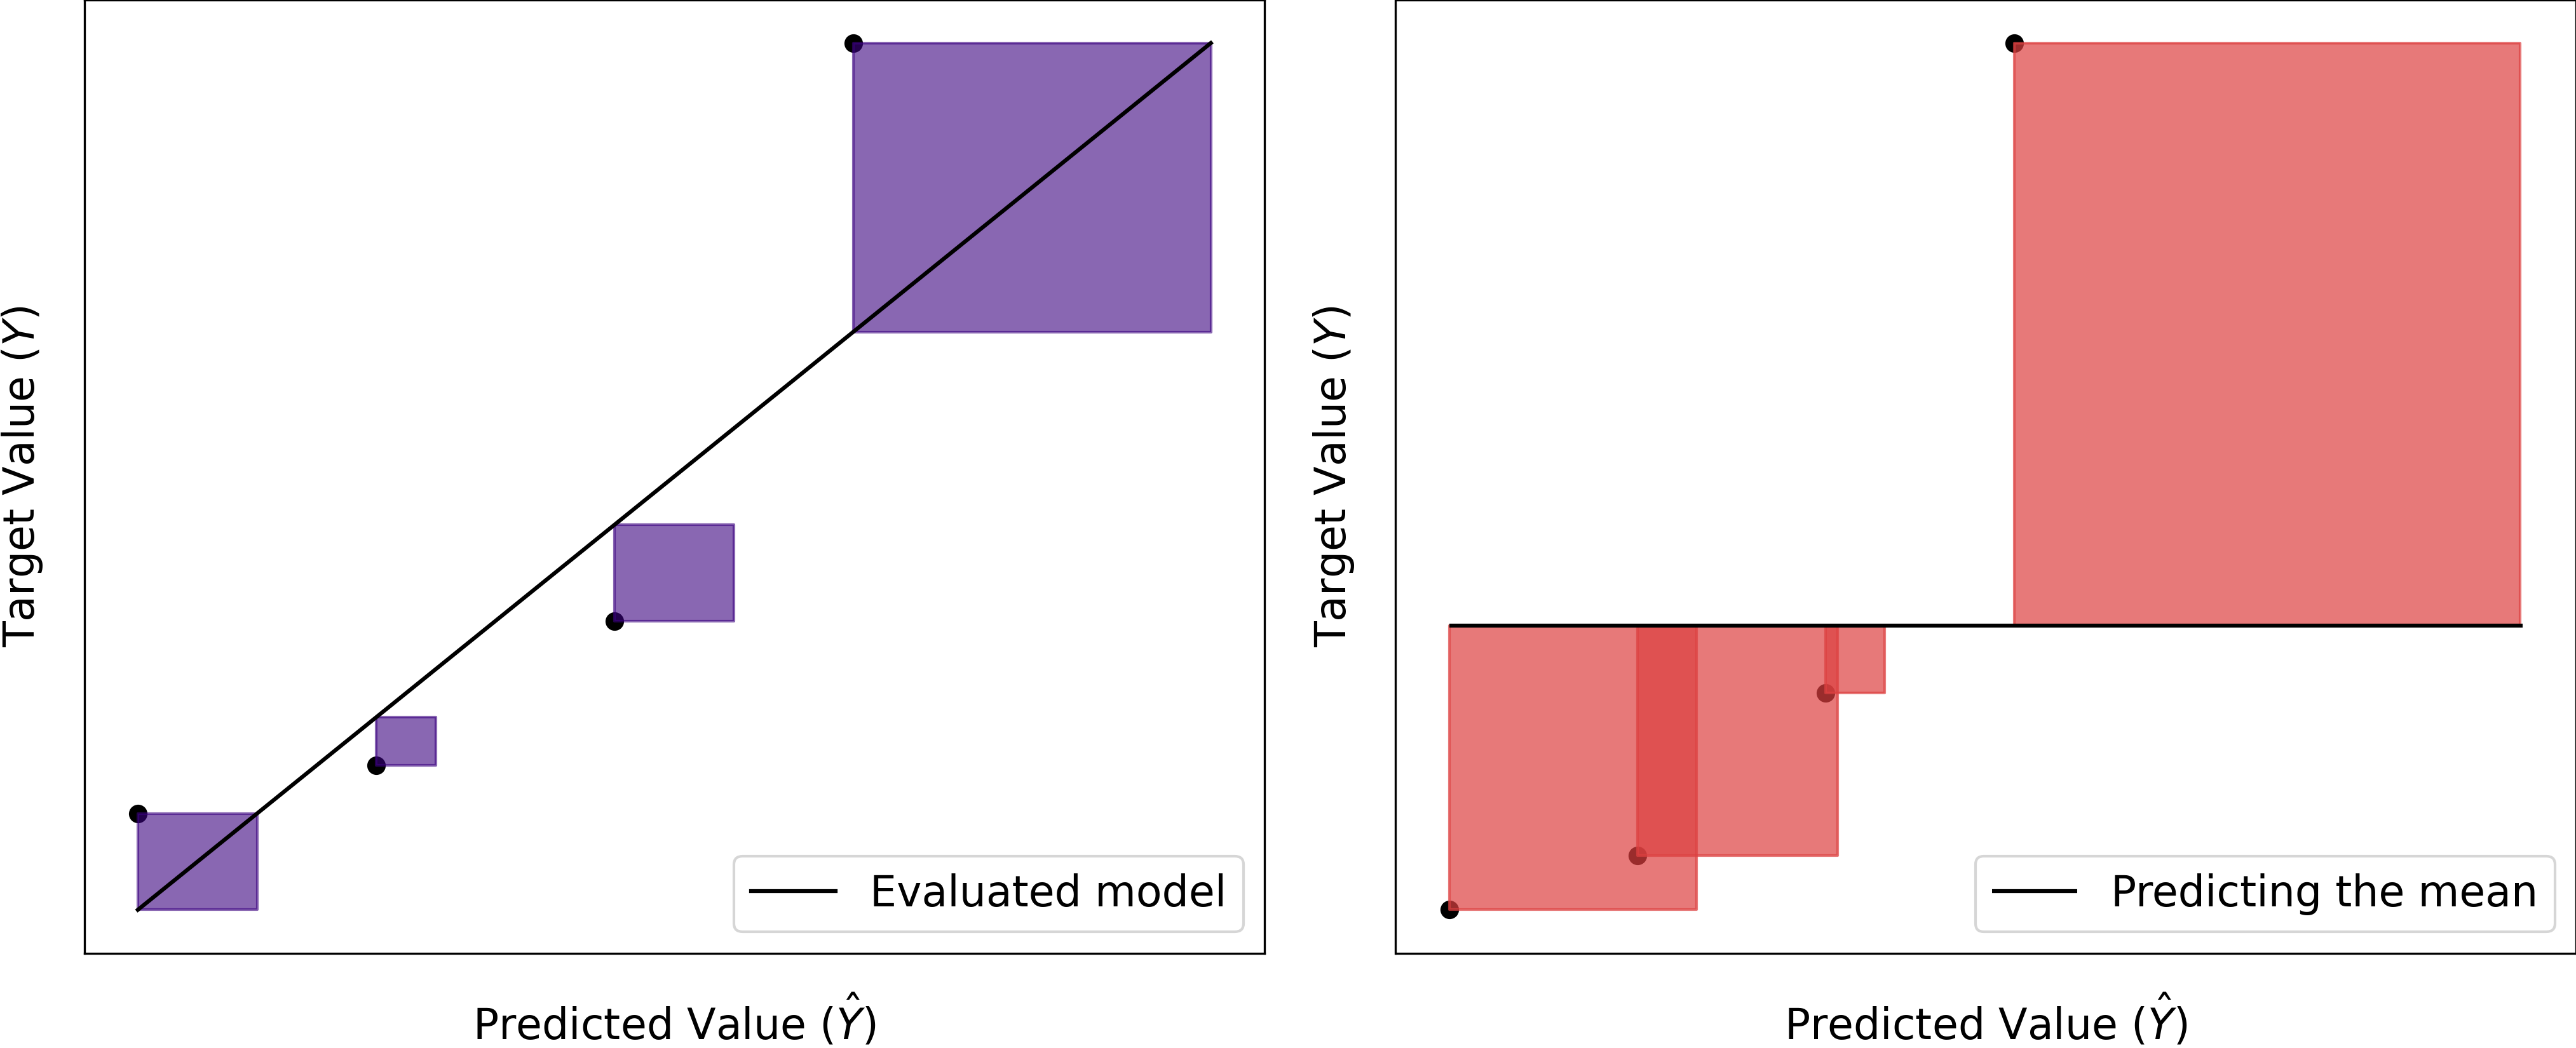
\includegraphics[width=\textwidth]{figures/R2_explained.png}
    % \caption{Caption}
    \label{fig1}
\end{figure*}

\begin{wrapfigure}{r}{0.5\textwidth}
    \centering
    \vspace{-10pt} % Adjust vertical alignment if needed
    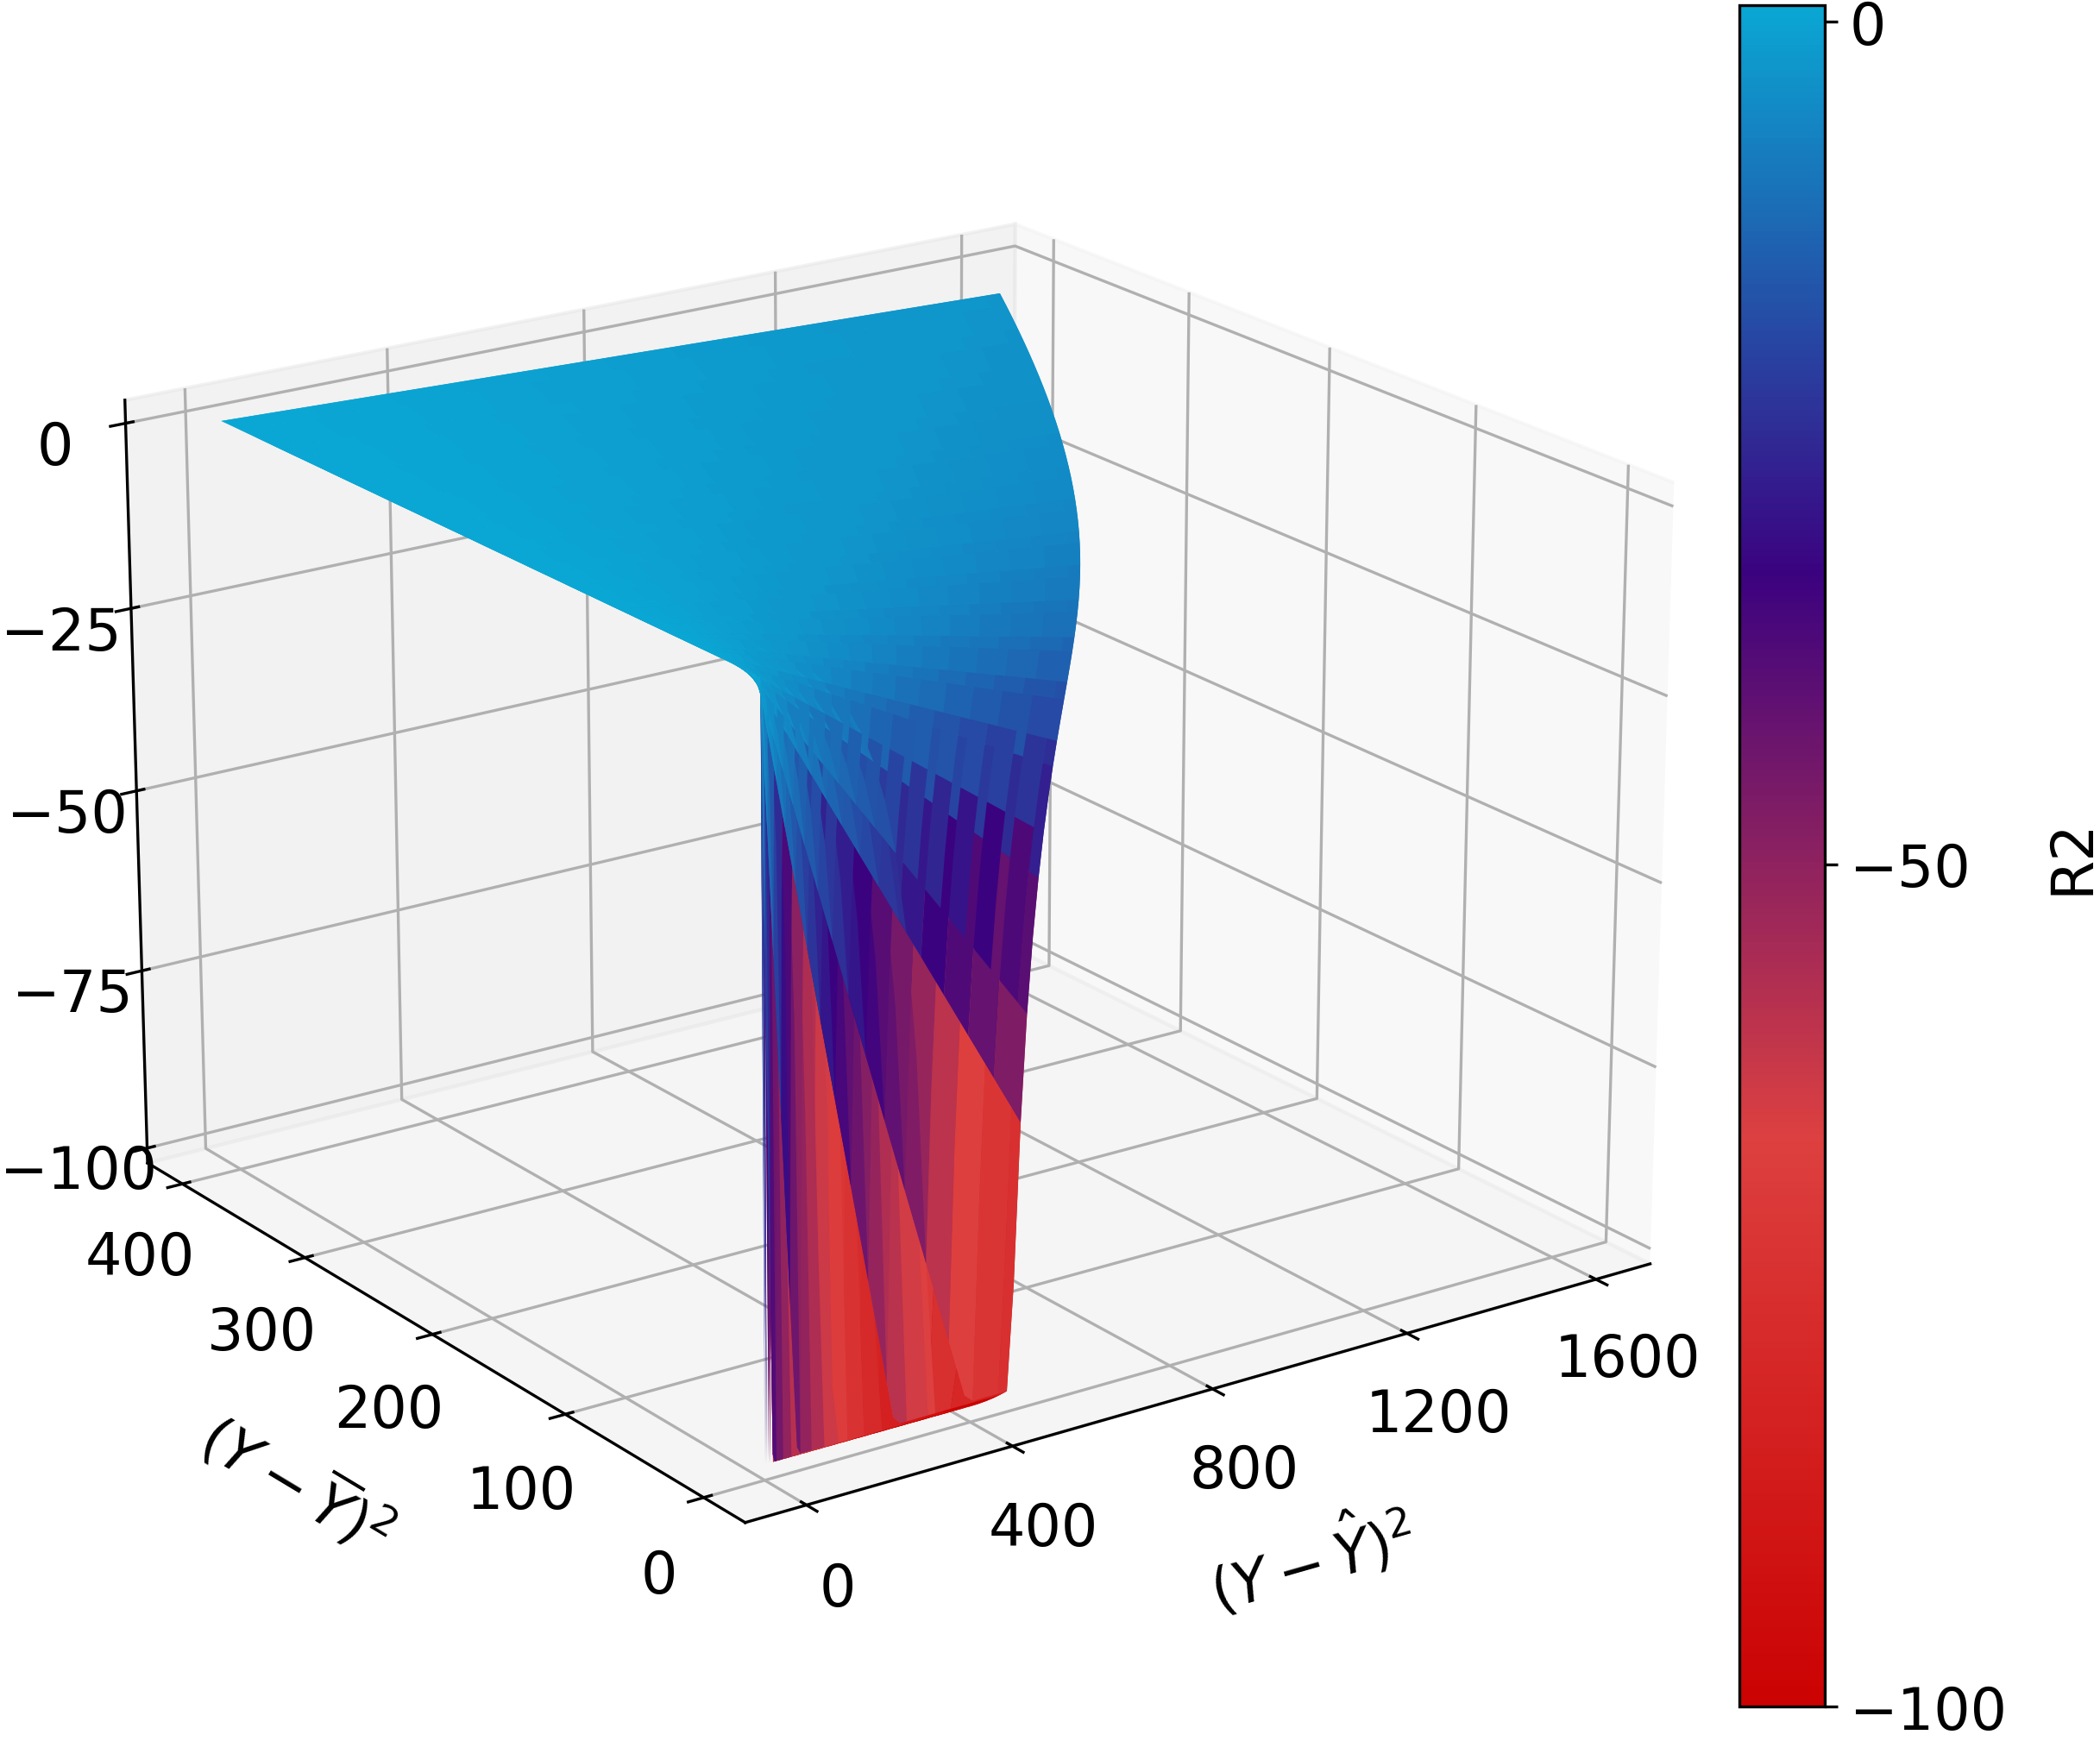
\includegraphics[width=0.45\textwidth]{figures/R2_3d_surface.png} % Your figure goes here
    \vspace{-10pt} % Adjust vertical alignment if needed
\end{wrapfigure}

% Left text with the image on the right
\textbf{Figure 2.15 R-Squared.} \textbf{Top:} The
areas of the purple squares
represent the MSE of the
evaluated model. While, the areas
of the red squares represent the
MSE of a model that always
predicts the mean. R-squared
can be written as $R^2 = 1-\frac{\color{violet!50}MSE_{model}}{\color{red!50}MSE_{baseline}}$\\
\textbf{Right:} R-squared quickly drops
into the negative region in cases
where the mean is a better
predictor than the evaluated
model.


\orangebox{%
Did you know that...}
{
R-squared is more than 100 years old; it was introduced by geneticist Sewall Wright in 1921.
}


\textbf{R-squared alternatives and other metrics to look for}

Other metrics commonly explored alongside R-squared are Adjusted Rsquared, out-of-sample R-squared, Mean Absolute Error (MAE), Mean Squared Error (MSE), Root Mean Squared Error (RMSE), etc.










%-------------------- Section 2 -------------------------------
% \clearpage
% \thispagestyle{customstyle}
% \section{MAPE}
% \subsection{Mean Absolute Percentage Error}




% R-squared needs little introduction; it's featured in every statistics book. Also known as the coefficient of determination, it's commonly introduced as a measure that quantifies the amount of variability explained by the regression model.

% \begin{center}
% \tikz{
% \node[inner sep=2pt, font=\Large] (a) {
% {
% $\displaystyle
% R^2 = 1 - \frac{\sum_{t=1}^n (Y_t - {\color{violet!50!blue}\hat{Y}_t})^2}{\sum_{t=1}^n ({\color{cyan}Y_t} - {\color{teal!70!green}\bar{Y}})^2}
% $
% }
% };

% \draw[-latex,violet!50!blue, semithick] ($(a.north)+(2.1,0)$) to[bend left=15] node[pos=1, right] {Predicted value} +(1,.5); 
% \draw[-latex,teal!70!green, semithick] ($(a.south)+(2.1,0.1)$) to[bend right=15] node[pos=1, right] {Mean of targets} +(1,-.5); 
% \draw[-latex,cyan, semithick] ($(a.south)+(1,0.1)$) to[bend left=15] node[pos=1, left] {Target value} +(-1,-.5); 
% }
% \end{center}

% However, it may be easier to think of R-squared as a way to scale MSE between a perfect model and one that always predicts the mean. A score of 1.0 means $Y_t$ and $\hat{Y}_t$ are equal. Despite its name, R-squared can be negative if the model performs worse than just predicting the mean.

% \textbf{When to use R-squared?}

% R-squared can be more intuitive than MAE, MSE, RMSE, and other scale-dependent metrics since it can be expressed as a percentage, whereas the latter have arbitrary ranges.

% \coloredboxes{
% \item Easy Interpretation. Especially when interpreted as a scaled MSE.
% \item R-squared is widely accepted in statistical analysis and research, making it a standard choice for evaluating model performance.
% }
% {
% \item Just like MSE, R-squared can be sensitive to outliers, as large errors have a greater impact.
% \item Be cautious about which value of $\bar{Y}$ to use. Most implementations default to $\bar{Y}_{\text {test }}$ which can lead to information leakage. It is advisable to use $\bar{Y}_{\text {train }}$ instead.
% }


% \clearpage
% \thispagestyle{customstyle2}


% \begin{figure*}[ht!]
%     \centering
%     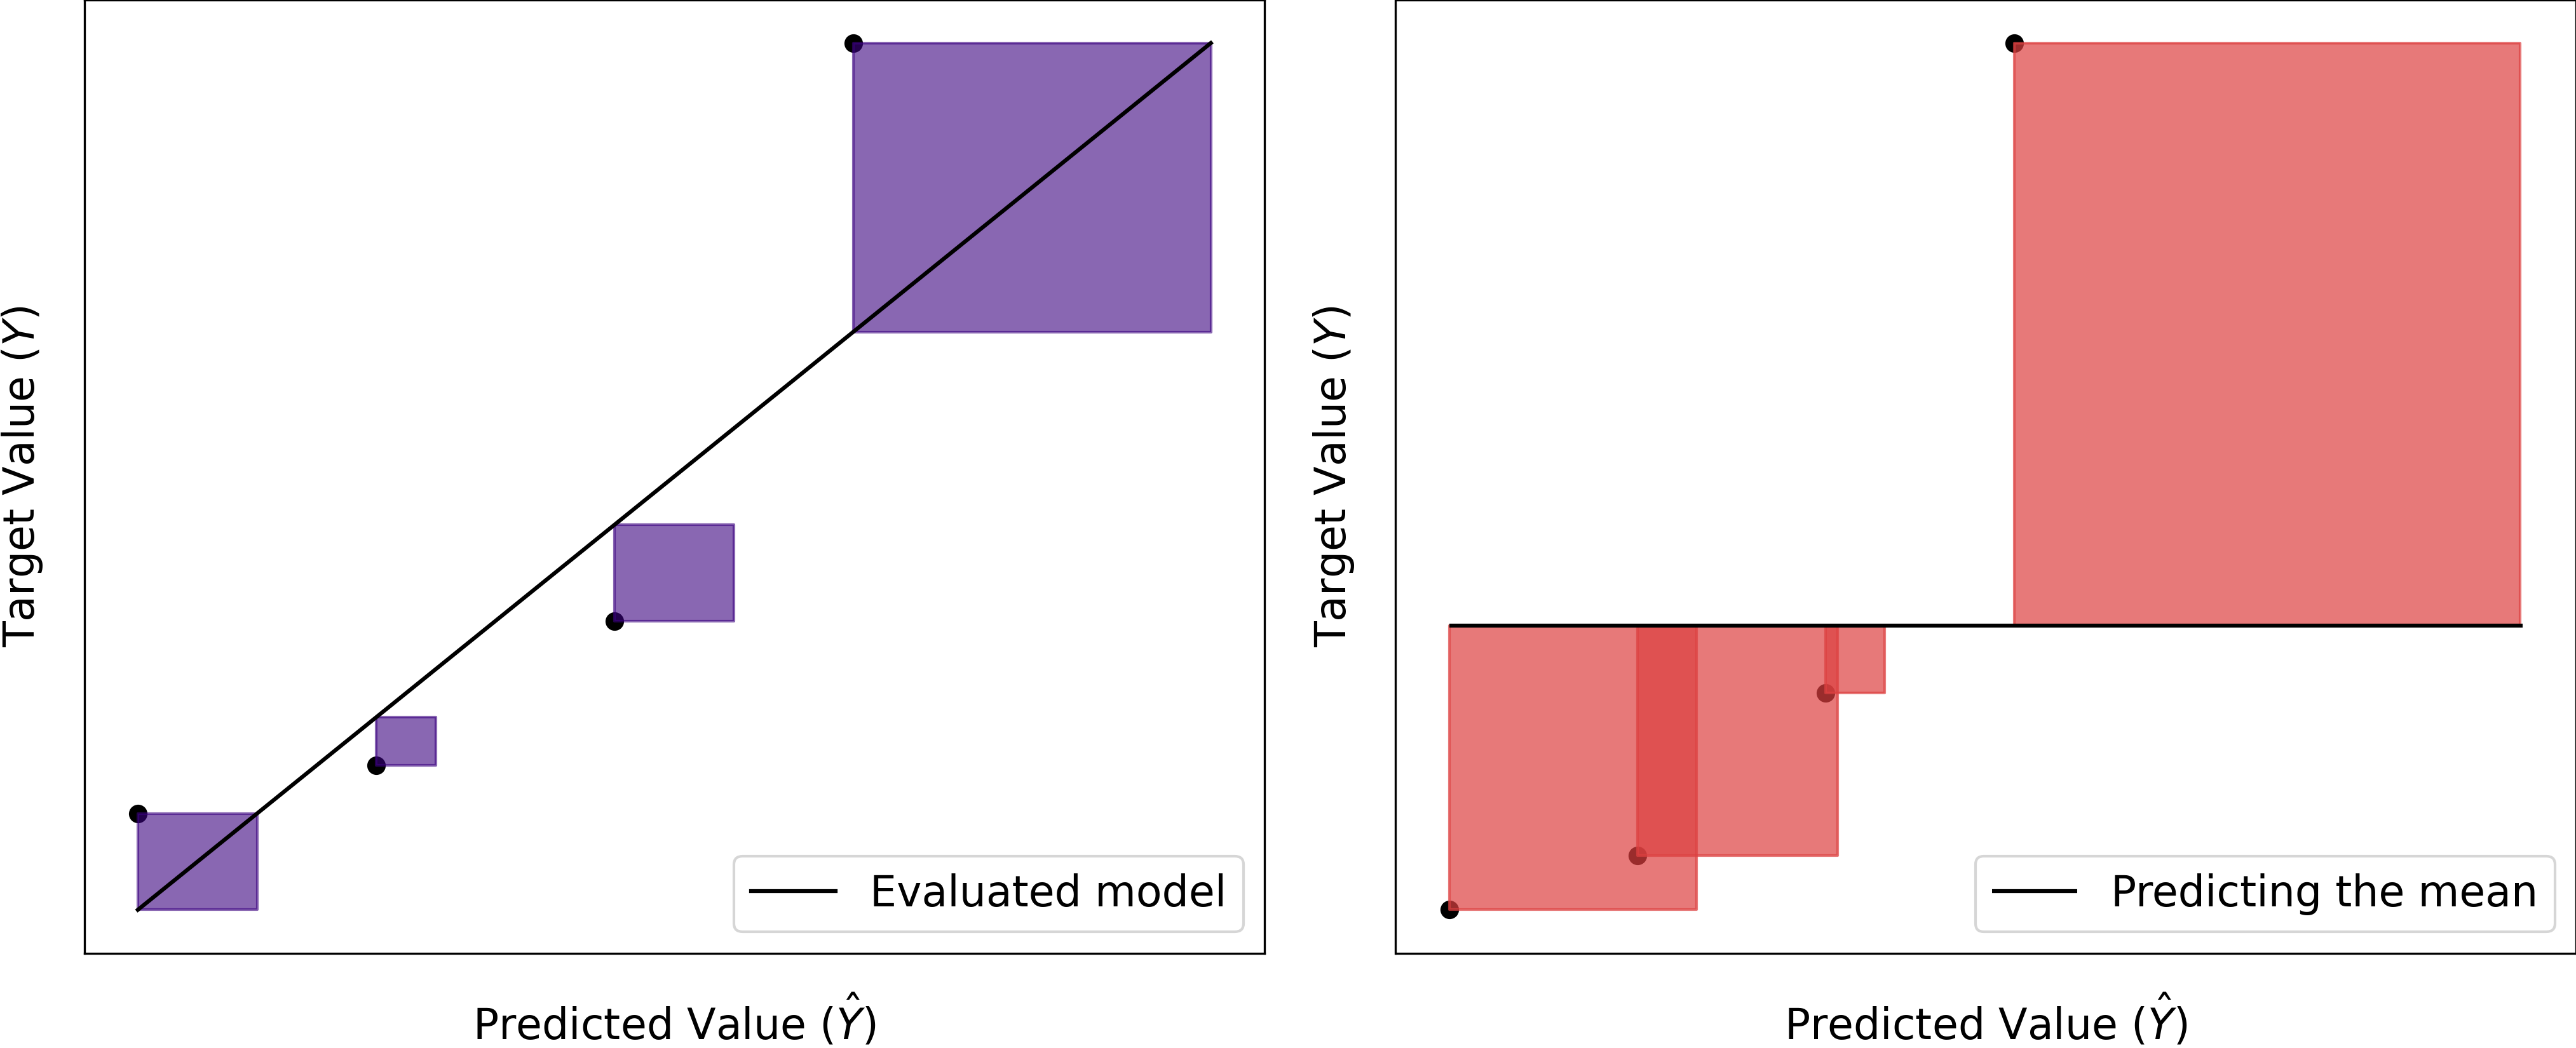
\includegraphics[width=\textwidth]{figures/R2_explained.png}
%     % \caption{Caption}
%     \label{fig1}
% \end{figure*}

% \begin{wrapfigure}{r}{0.5\textwidth}
%     \centering
%     \vspace{-10pt} % Adjust vertical alignment if needed
%     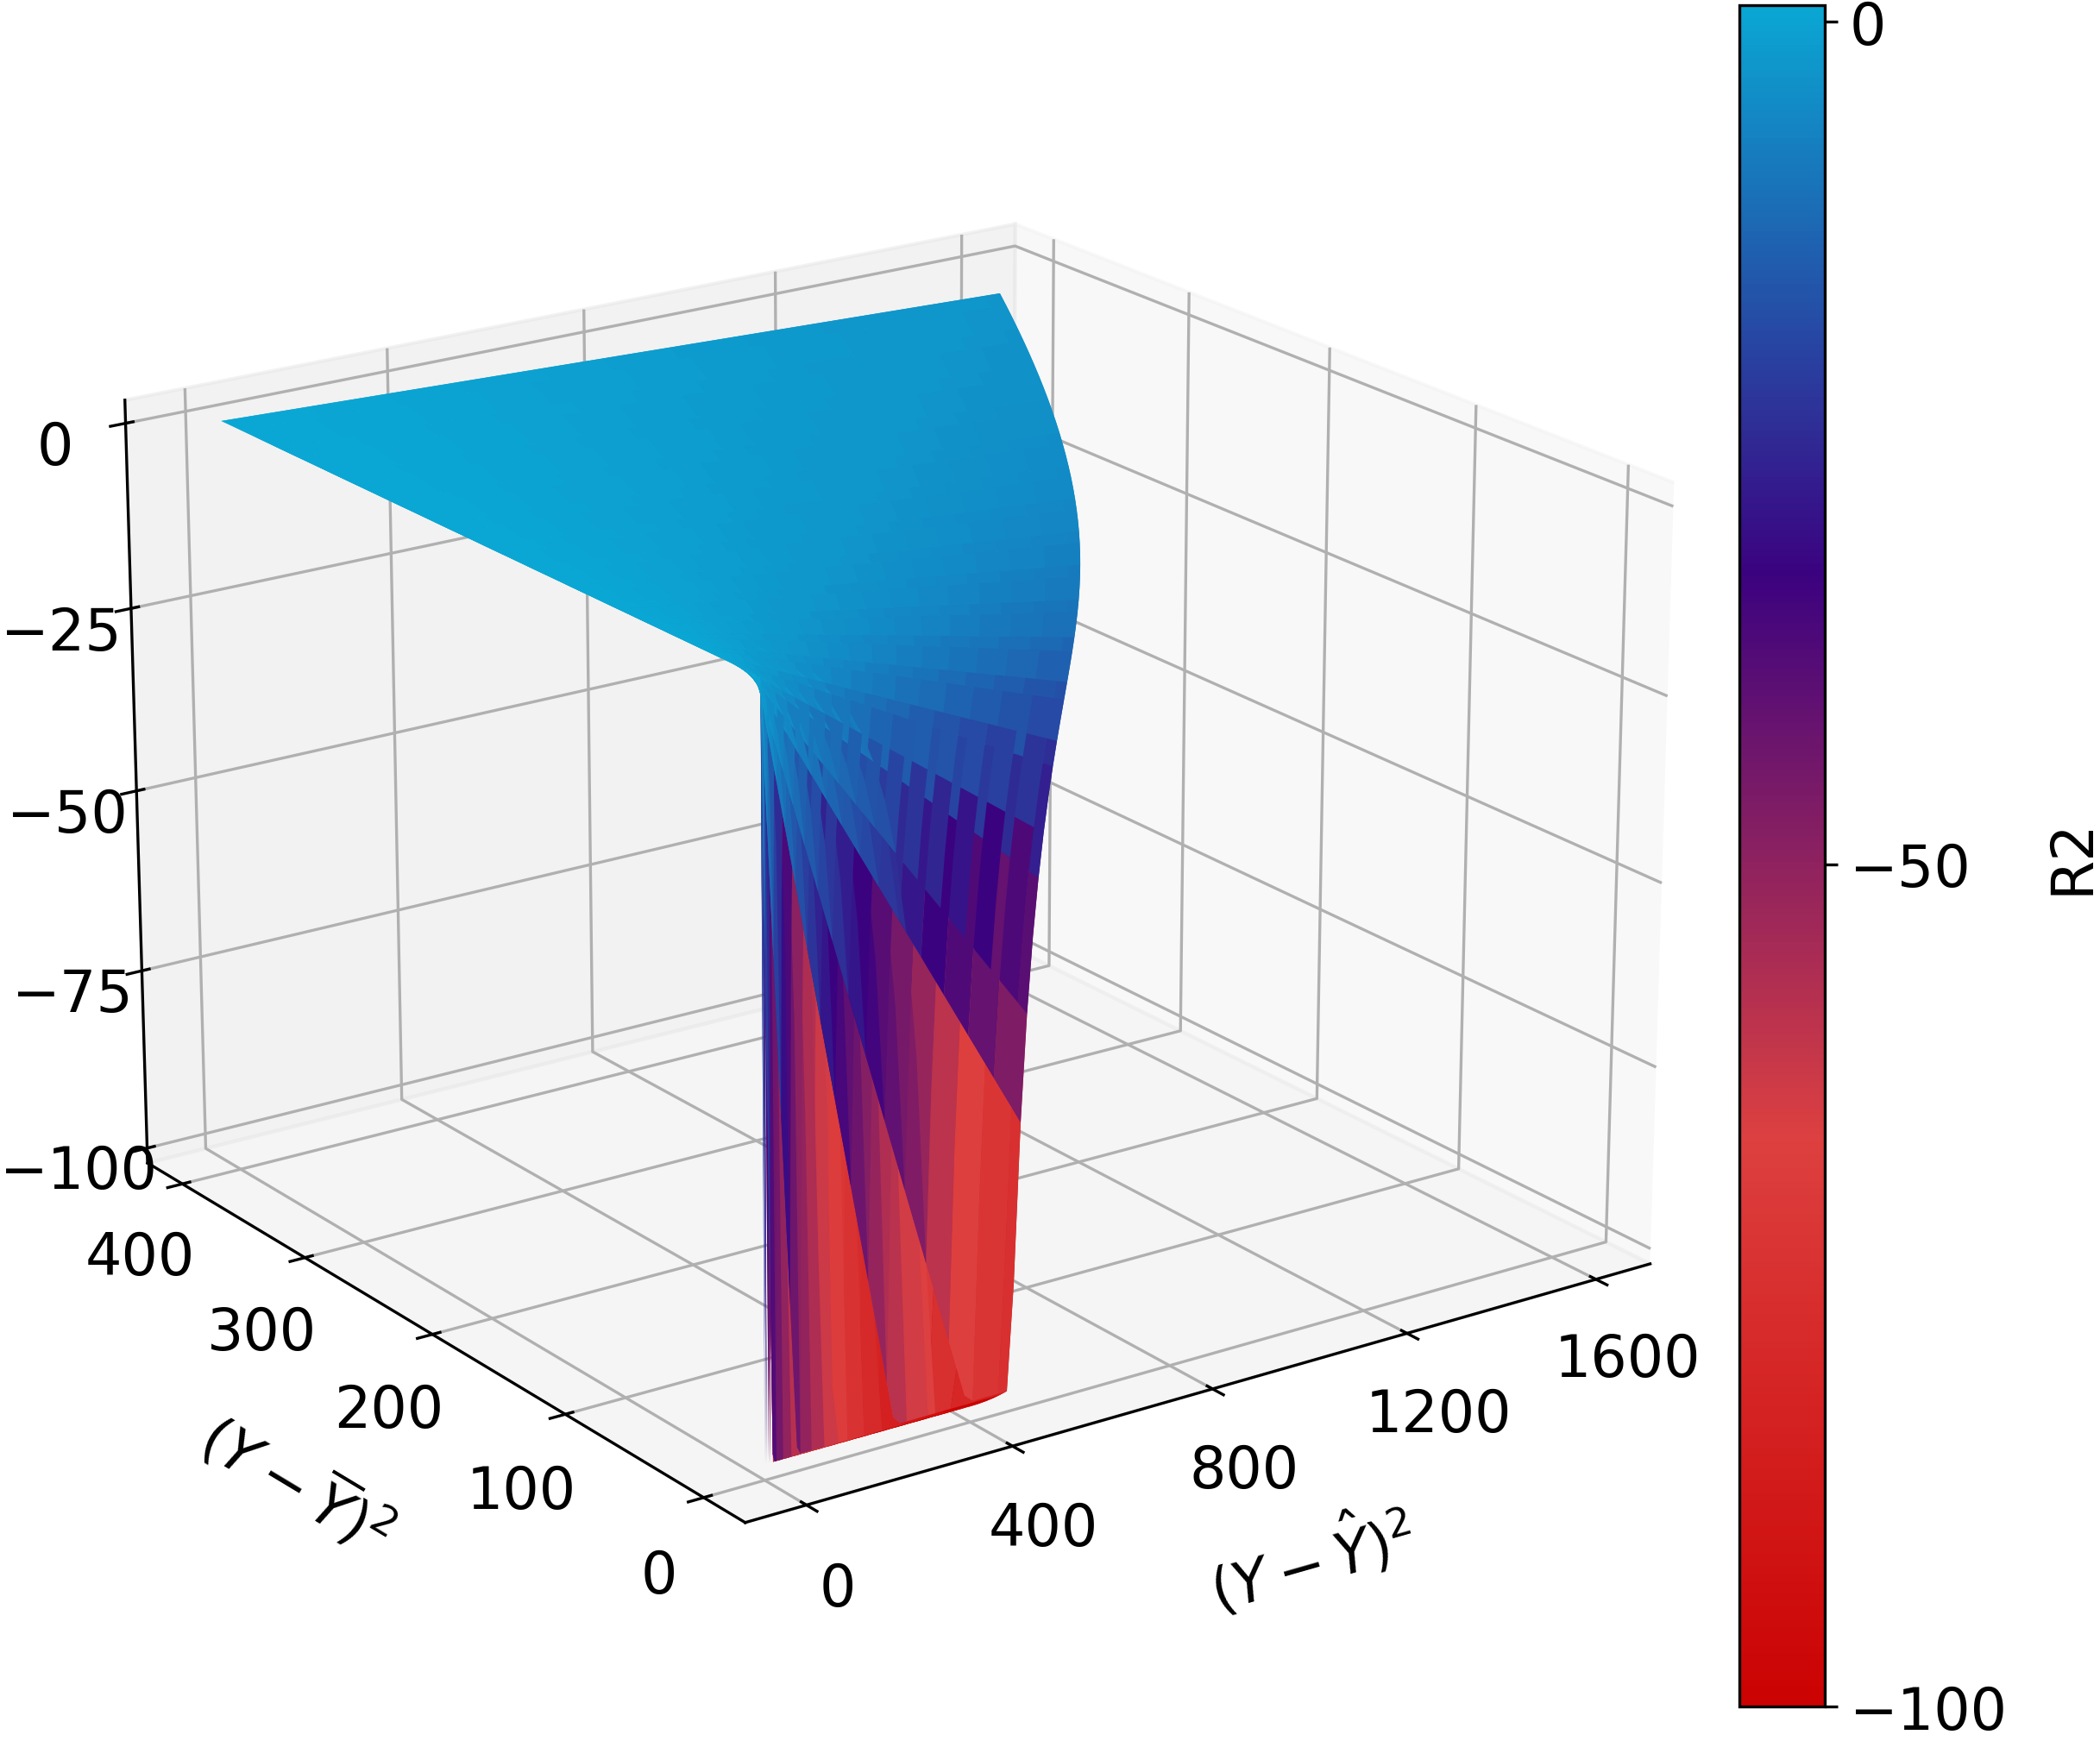
\includegraphics[width=0.45\textwidth]{figures/R2_3d_surface.png} % Your figure goes here
%     \vspace{-10pt} % Adjust vertical alignment if needed
% \end{wrapfigure}

% % Left text with the image on the right
% \textbf{Figure 2.15 R-Squared.} \textbf{Top:} The
% areas of the purple squares
% represent the MSE of the
% evaluated model. While, the areas
% of the red squares represent the
% MSE of a model that always
% predicts the mean. R-squared
% can be written as $R^2 = 1-\frac{\color{violet!50}MSE_{model}}{\color{red!50}MSE_{baseline}}$\\
% \textbf{Right:} R-squared quickly drops
% into the negative region in cases
% where the mean is a better
% predictor than the evaluated
% model.


% \orangebox{%
% Did you know that...}
% {
% R-squared is more than 100 years old; it was introduced by geneticist Sewall Wright in 1921.
% }


% \textbf{R-squared alternatives and other metrics to look for}

% Other metrics commonly explored alongside R-squared are Adjusted Rsquared, out-of-sample R-squared, Mean Absolute Error (MAE), Mean Squared Error (MSE), Root Mean Squared Error (RMSE), etc.
\chapter{Classification}

% ---------- Confusion Matrix ----------
\thispagestyle{classificationstyle}
\section{Confusion Matrix}
\subsection{Confusion Matrix}

% ---------- FPR ----------
\clearpage
\section{FPR}
\subsection{False Positive Rate}
\thispagestyle{classificationstyle}

The False Positive Rate (FPR), also known as the false alarm ratio or fall-out, measures how often negative instances are incorrectly classified as positive in binary classification.

\begin{center}
\tikz{
\node[inner sep=2pt, font=\Large] (a) {
{
$\displaystyle
FPR = \frac{{\color{cyan}FP}}{{\color{cyan}FP} + {{\color{nmlpurple}TN}}}
$
}
};
\draw[-latex,cyan, semithick] ($(a.north)+(1.3,0.05)$) to[bend left=15] node[pos=1, right] {False positives} +(1,.5); 
% \draw[-latex,teal!70!green, semithick] ($(a.south)+(2.1,0.1)$) to[bend right=15] node[pos=1, right] {Mean of targets} +(1,-.5); 
\draw[-latex,nmlpurple, semithick] ($(a.south)+(1.5,-0.05)$) to[bend left=15] node[pos=1, left] {True negatives} +(-1,-.5); 
}
\end{center}

FPR ranges from 0 (no false alarms) to 1 (all predicted positives are incorrect). FPR can also be interpreted as the probability that a negative instance will be incorrectly identified as positive.

\textbf{When to use FPR?}

Use FPR when you need to evaluate how well a classifier avoids false positives, especially when false positives have significant costs, like in medical diagnostics or security systems. It's also useful for understanding the trade-off between true positive rate (sensitivity) and false positive rate.

\coloredboxes{
\item It provides a clear and intuitive measure of a classifier's false positive performance.
\item It helps identify scenarios where the classifier is overly sensitive and prone to false alarms.
}
{
\item FPR does not consider true positive instances.
\item FPR can be sensitive to class imbalance, as it may be easier to achieve a low FPR when the negative class is dominant.
\item FPR doesn't exist in isolation; it's often important to show its relationship with another key metric. (e.g., TPR, Precision, Recall).
}


\clearpage
\thispagestyle{customstyle}


\begin{figure*}[ht!]
    \centering
    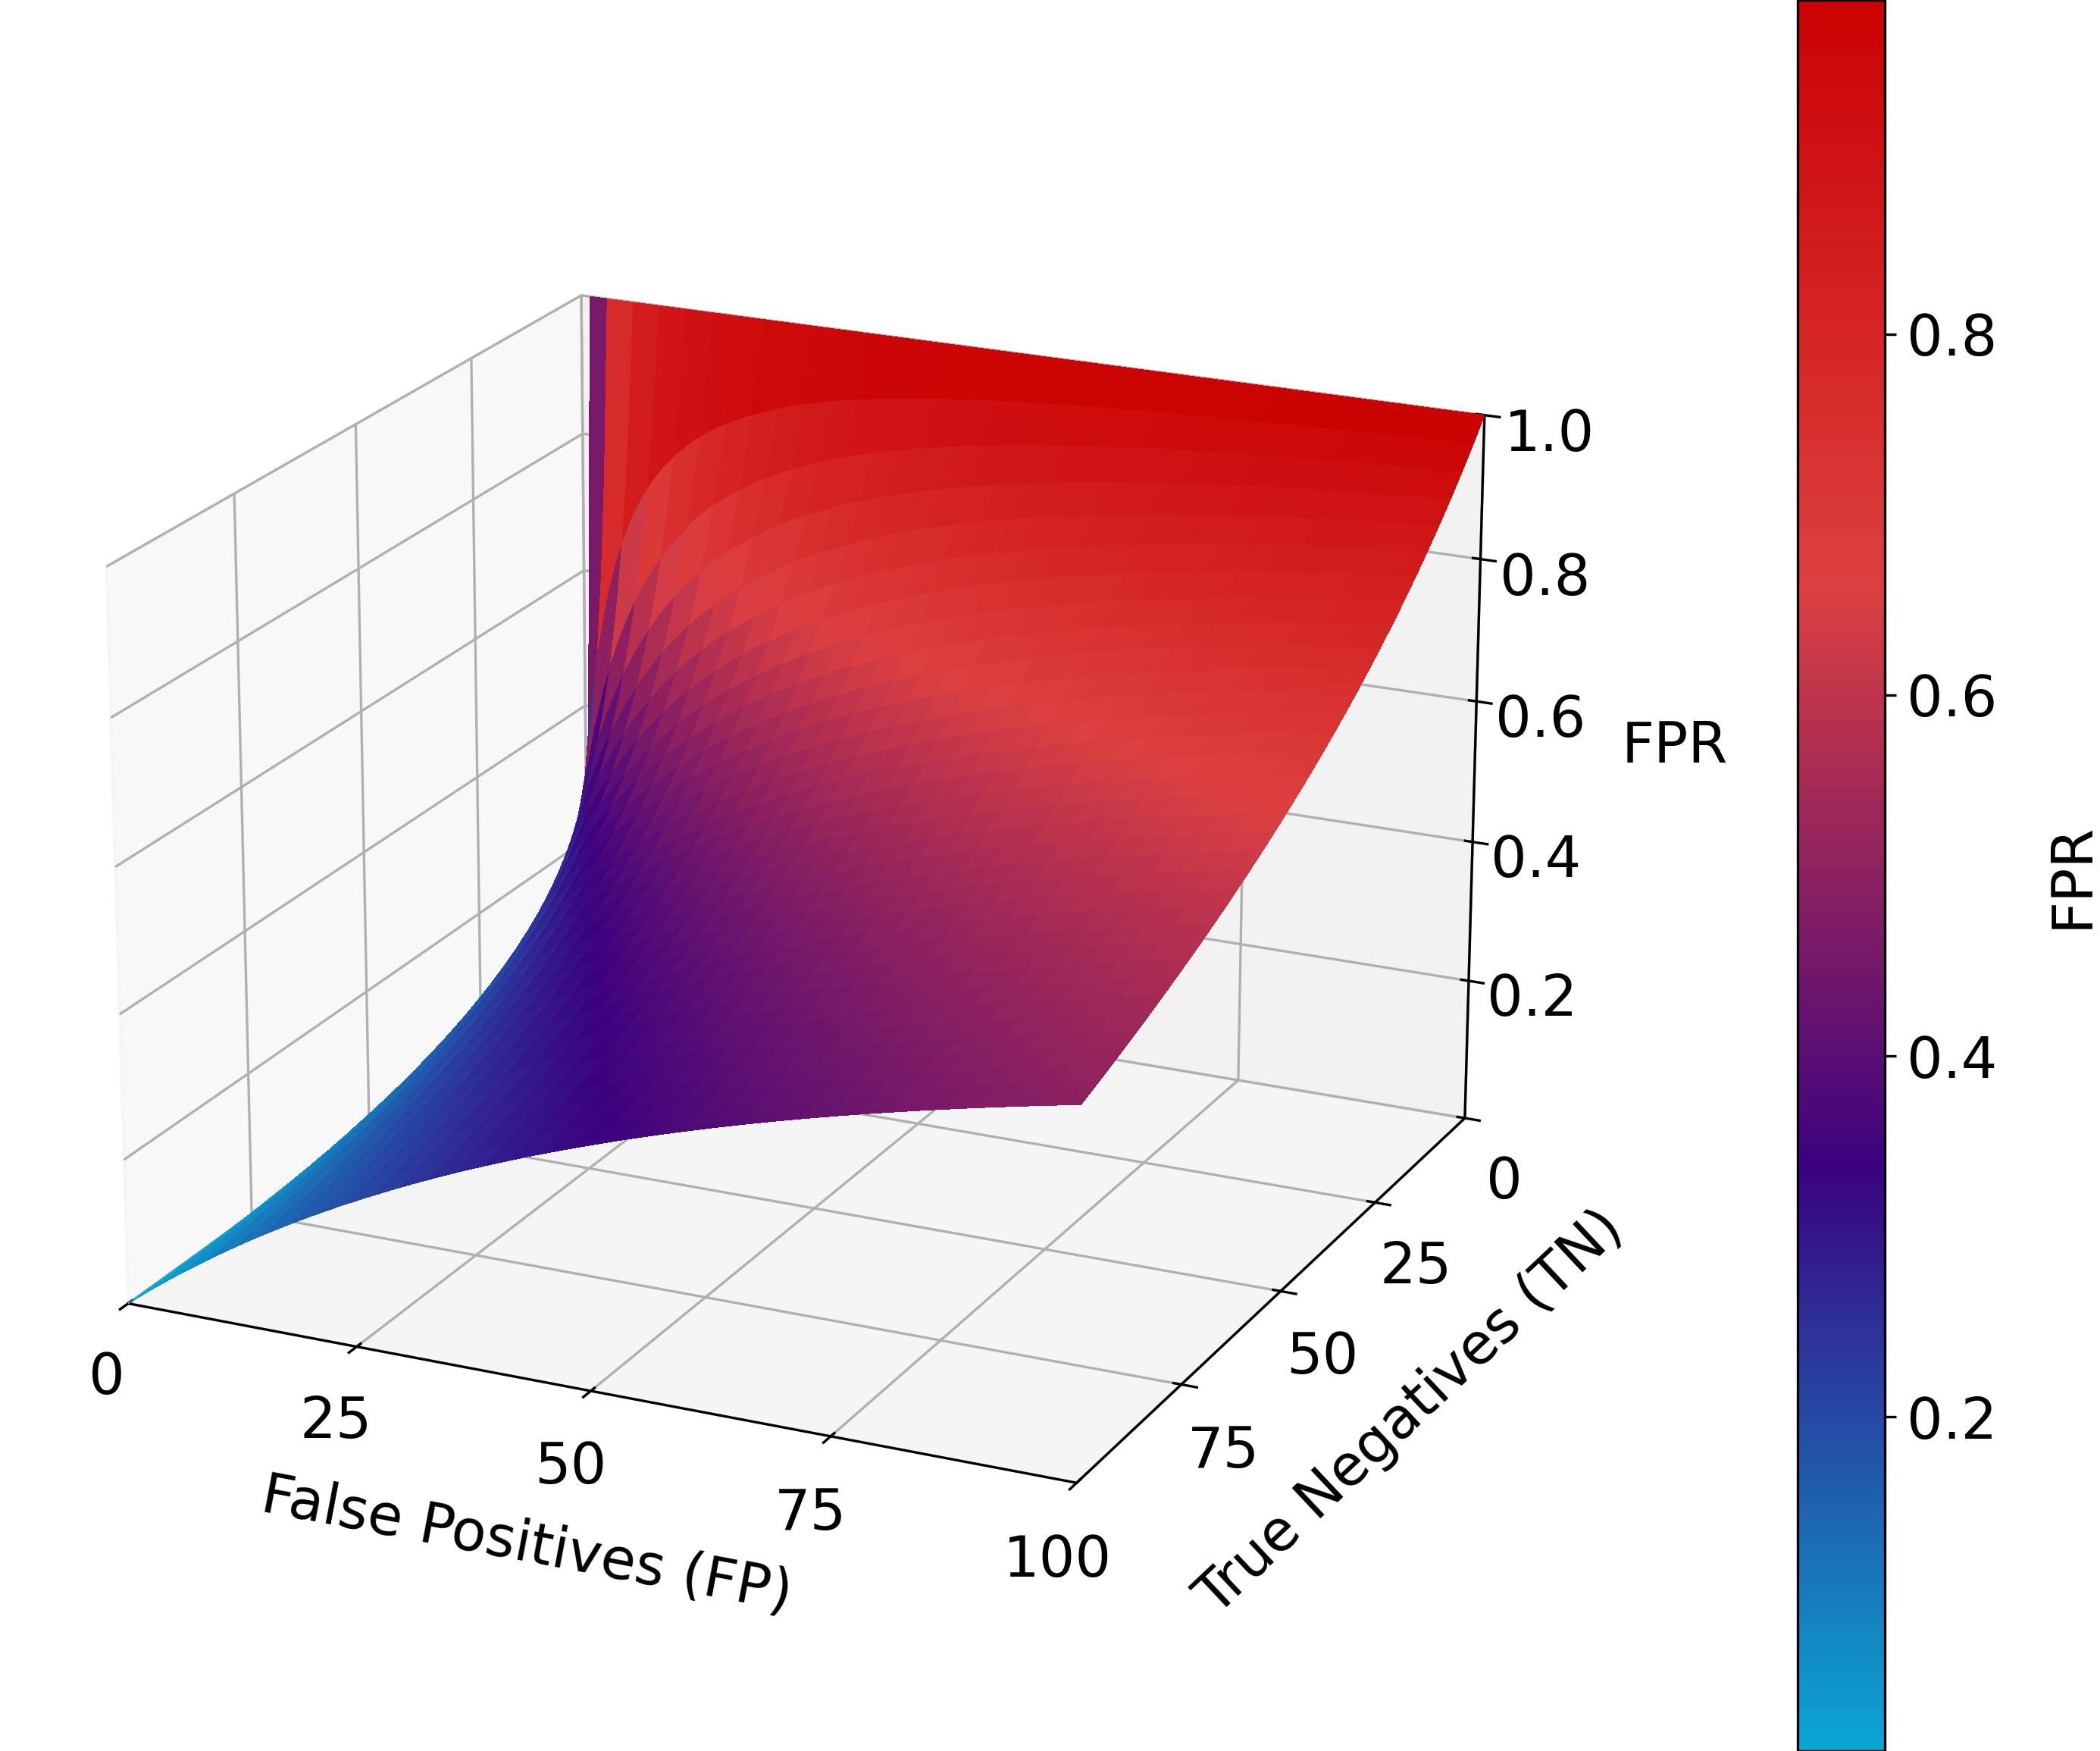
\includegraphics[width=0.7\textwidth]{figures/FPR_3d_surface.png}
    % \caption{Caption}
    \label{fig1}
\end{figure*}

\begin{wrapfigure}{r}{0.55\textwidth}
    \centering
    \vspace{-20pt} % Adjust vertical alignment if needed
    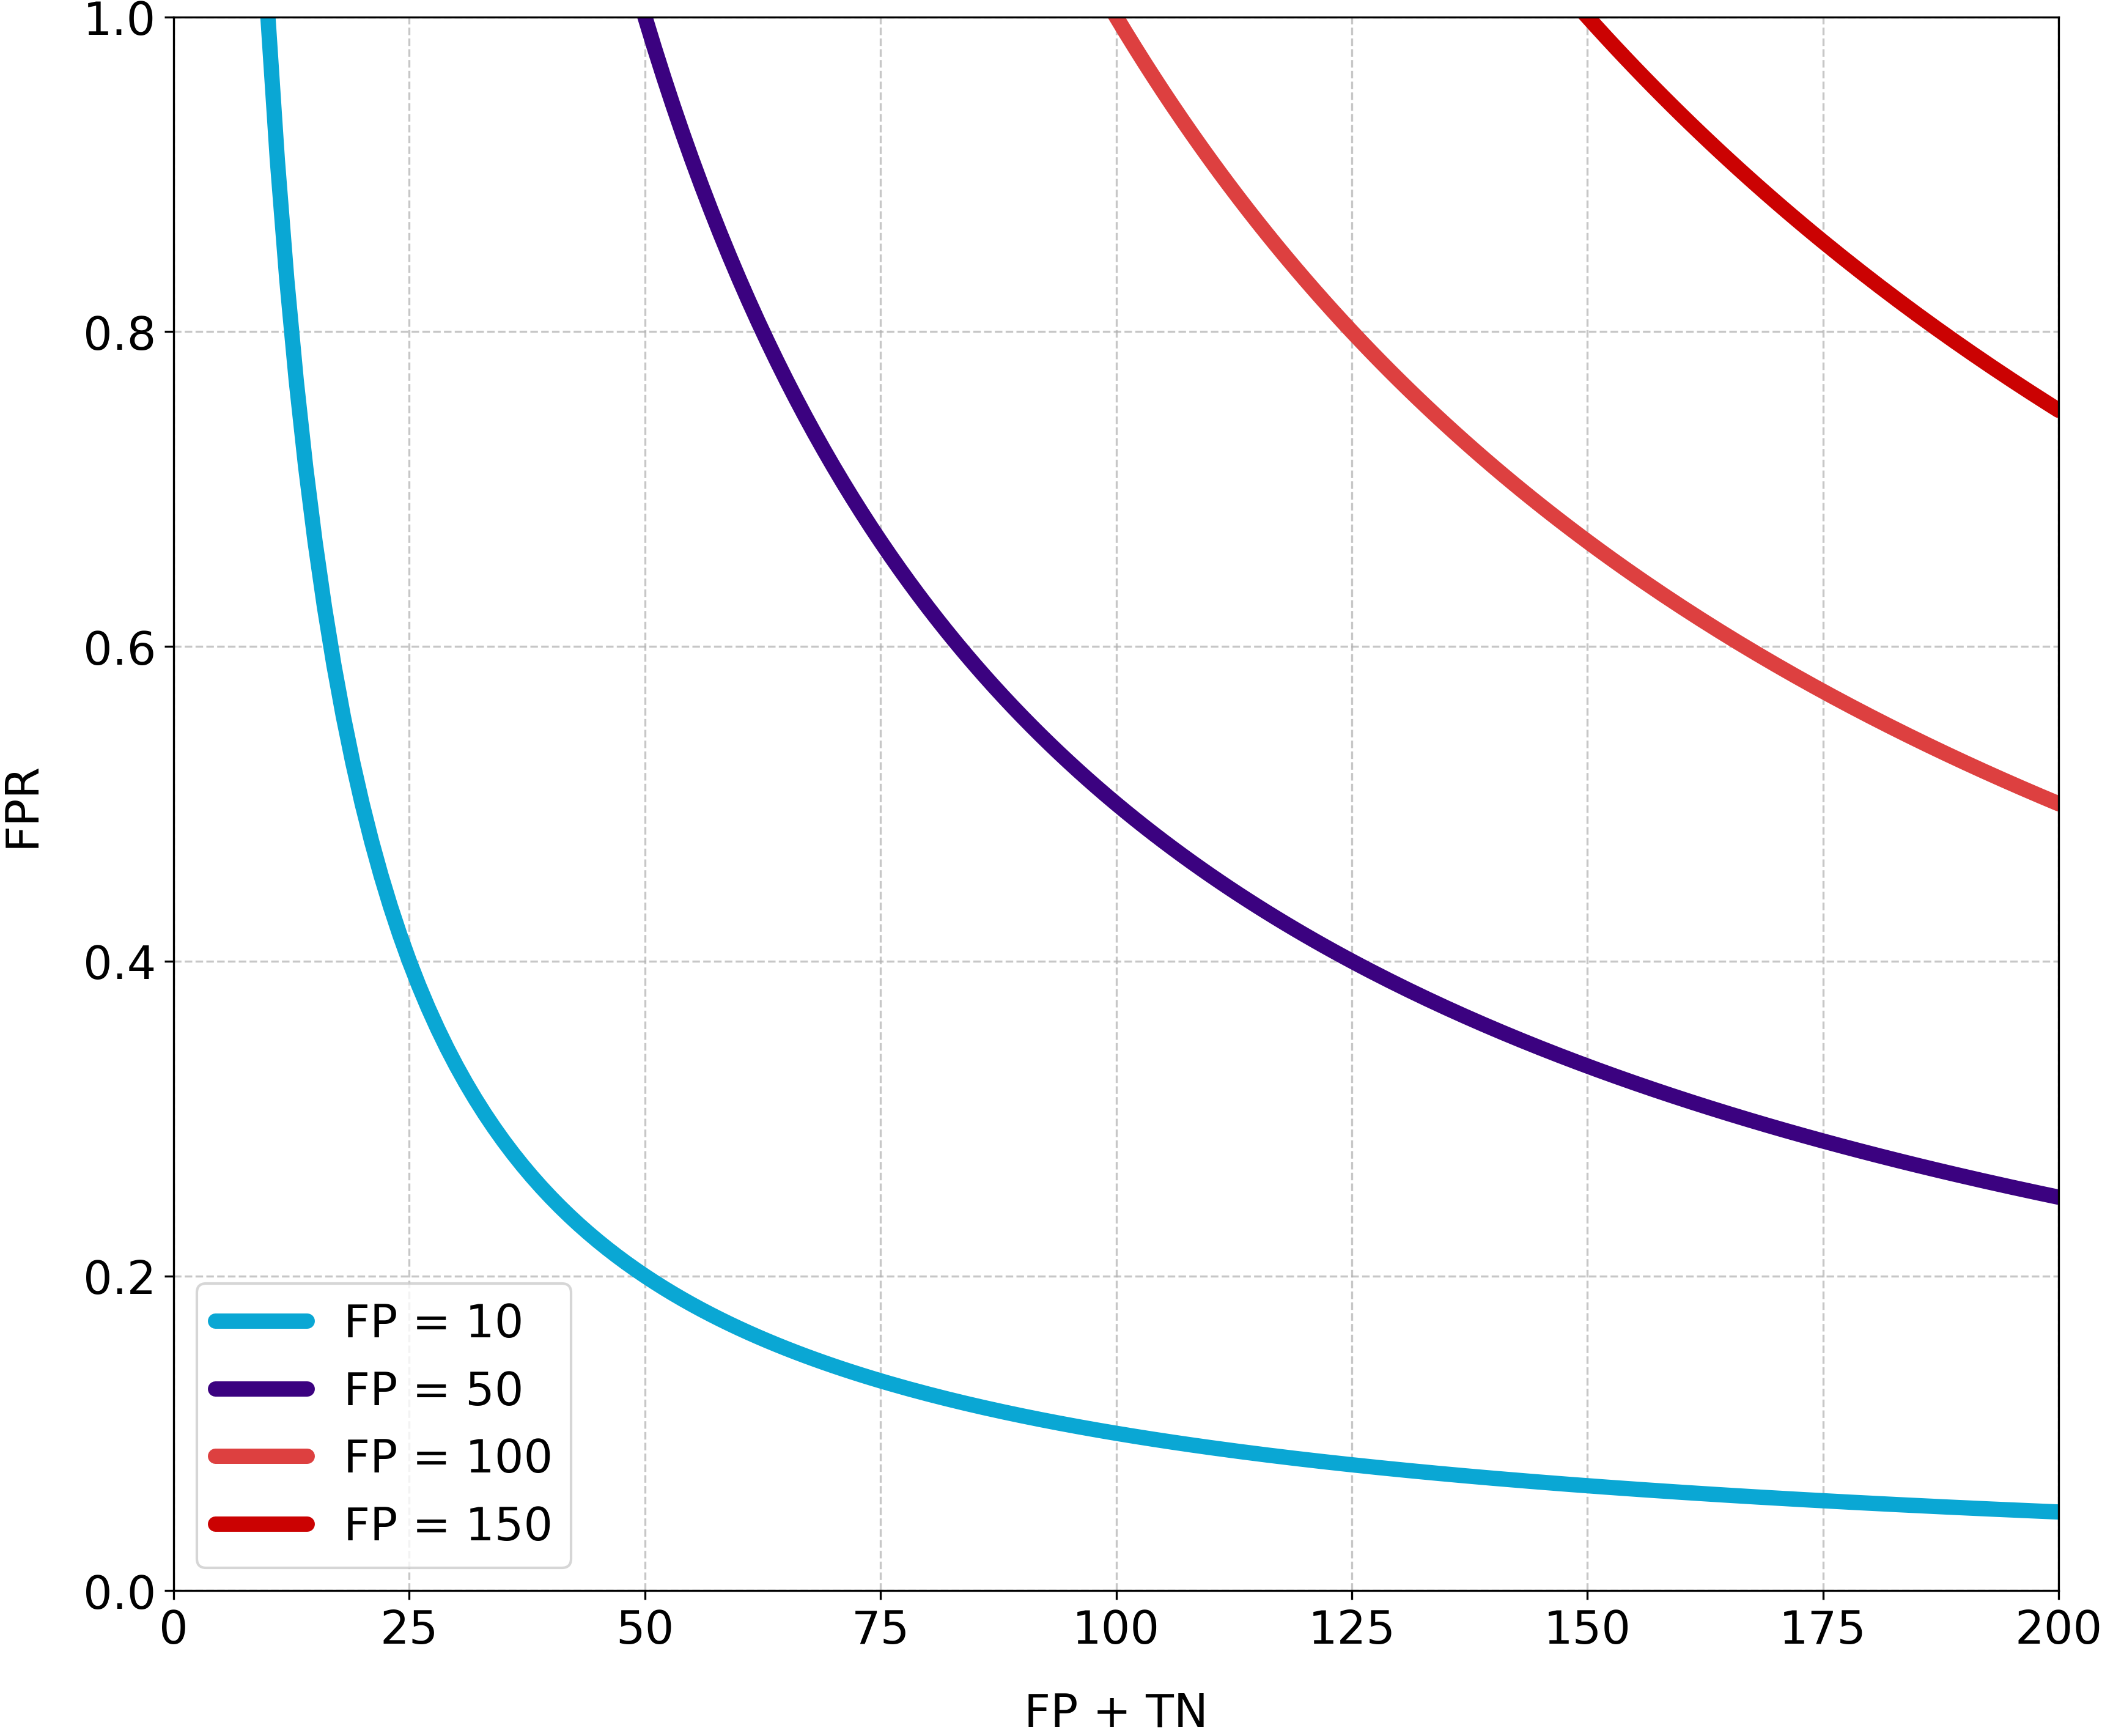
\includegraphics[width=0.5\textwidth]{figures/FPR_2d_line_plot.png} % Your figure goes here
\end{wrapfigure}

% Left text with the image on the right
\textbf{Figure 3.1 False Positive Rate.} 
\textbf{Top:}
3D surface illustrating FPR's non-linear relationship with FP and TN. FPR is lowest (blue) when FP is low. It increases (red) as FP increases.
\textbf{Right:}
Shows how FPR decreases hyperbolically as total negative cases increase for fixed FP values. Lower FP maintains better FPR.


\orangebox{%
Did you know that...}
{
In the context of statistical hypothesis testing, the FPR is also known as the "type I error rate" or the probability of rejecting a true null hypothesis.
}

\textbf{FPR alternatives and related metrics}

Other metrics used alongside or instead of FPR include True Positive Rate (TPR), Precision, F1-Score, Receiver Operating Characteristic (ROC AUC), and Specificity.


% ---------- FNR ----------
\clearpage
\section{FNR}
\subsection{False Negative Rate}
\thispagestyle{classificationstyle}

The False Negative Rate (FNR), also known as the miss rate, measures the proportion of actual positive instances incorrectly classified as negative in binary classification.
\begin{center}
\tikz{
\node[inner sep=2pt, font=\Large] (a) {
{
$\displaystyle
FPR = \frac{{\color{cyan}FP}}{{\color{cyan}FP} + {{\color{nmlpurple}TN}}}
$
}
};
\draw[-latex,cyan, semithick] ($(a.north)+(1.3,0.05)$) to[bend left=15] node[pos=1, right] {False positives} +(1,.5); 
% \draw[-latex,teal!70!green, semithick] ($(a.south)+(2.1,0.1)$) to[bend right=15] node[pos=1, right] {Mean of targets} +(1,-.5); 
\draw[-latex,nmlpurple, semithick] ($(a.south)+(1.5,-0.05)$) to[bend left=15] node[pos=1, left] {True negatives} +(-1,-.5); 
}
\end{center}

FNR ranges from 0 (no false negatives) to 1 (all positive instances misclassified). It represents the probability that a positive instance will be incorrectly identified as negative.

\textbf{When to use FNR?}

Use FNR when the cost of missing positive cases is high (e.g., in medical diagnostics or fraud detection) or when you must balance false negatives and false positives.

\coloredboxes{
\item It directly measures the rate of missed positive cases.
\item It is critical in fields where false negatives have severe consequences.
\item Complements True Positive Rate (TPR) in assessing classifier performance.
}
{
\item It doesn't account for true negatives or false positives.
\item It can be misleading in highly imbalanced datasets.
\item It should be considered alongside other metrics for a comprehensive evaluation.
}


\clearpage
\thispagestyle{customstyle}


\begin{figure*}[ht!]
    \centering
    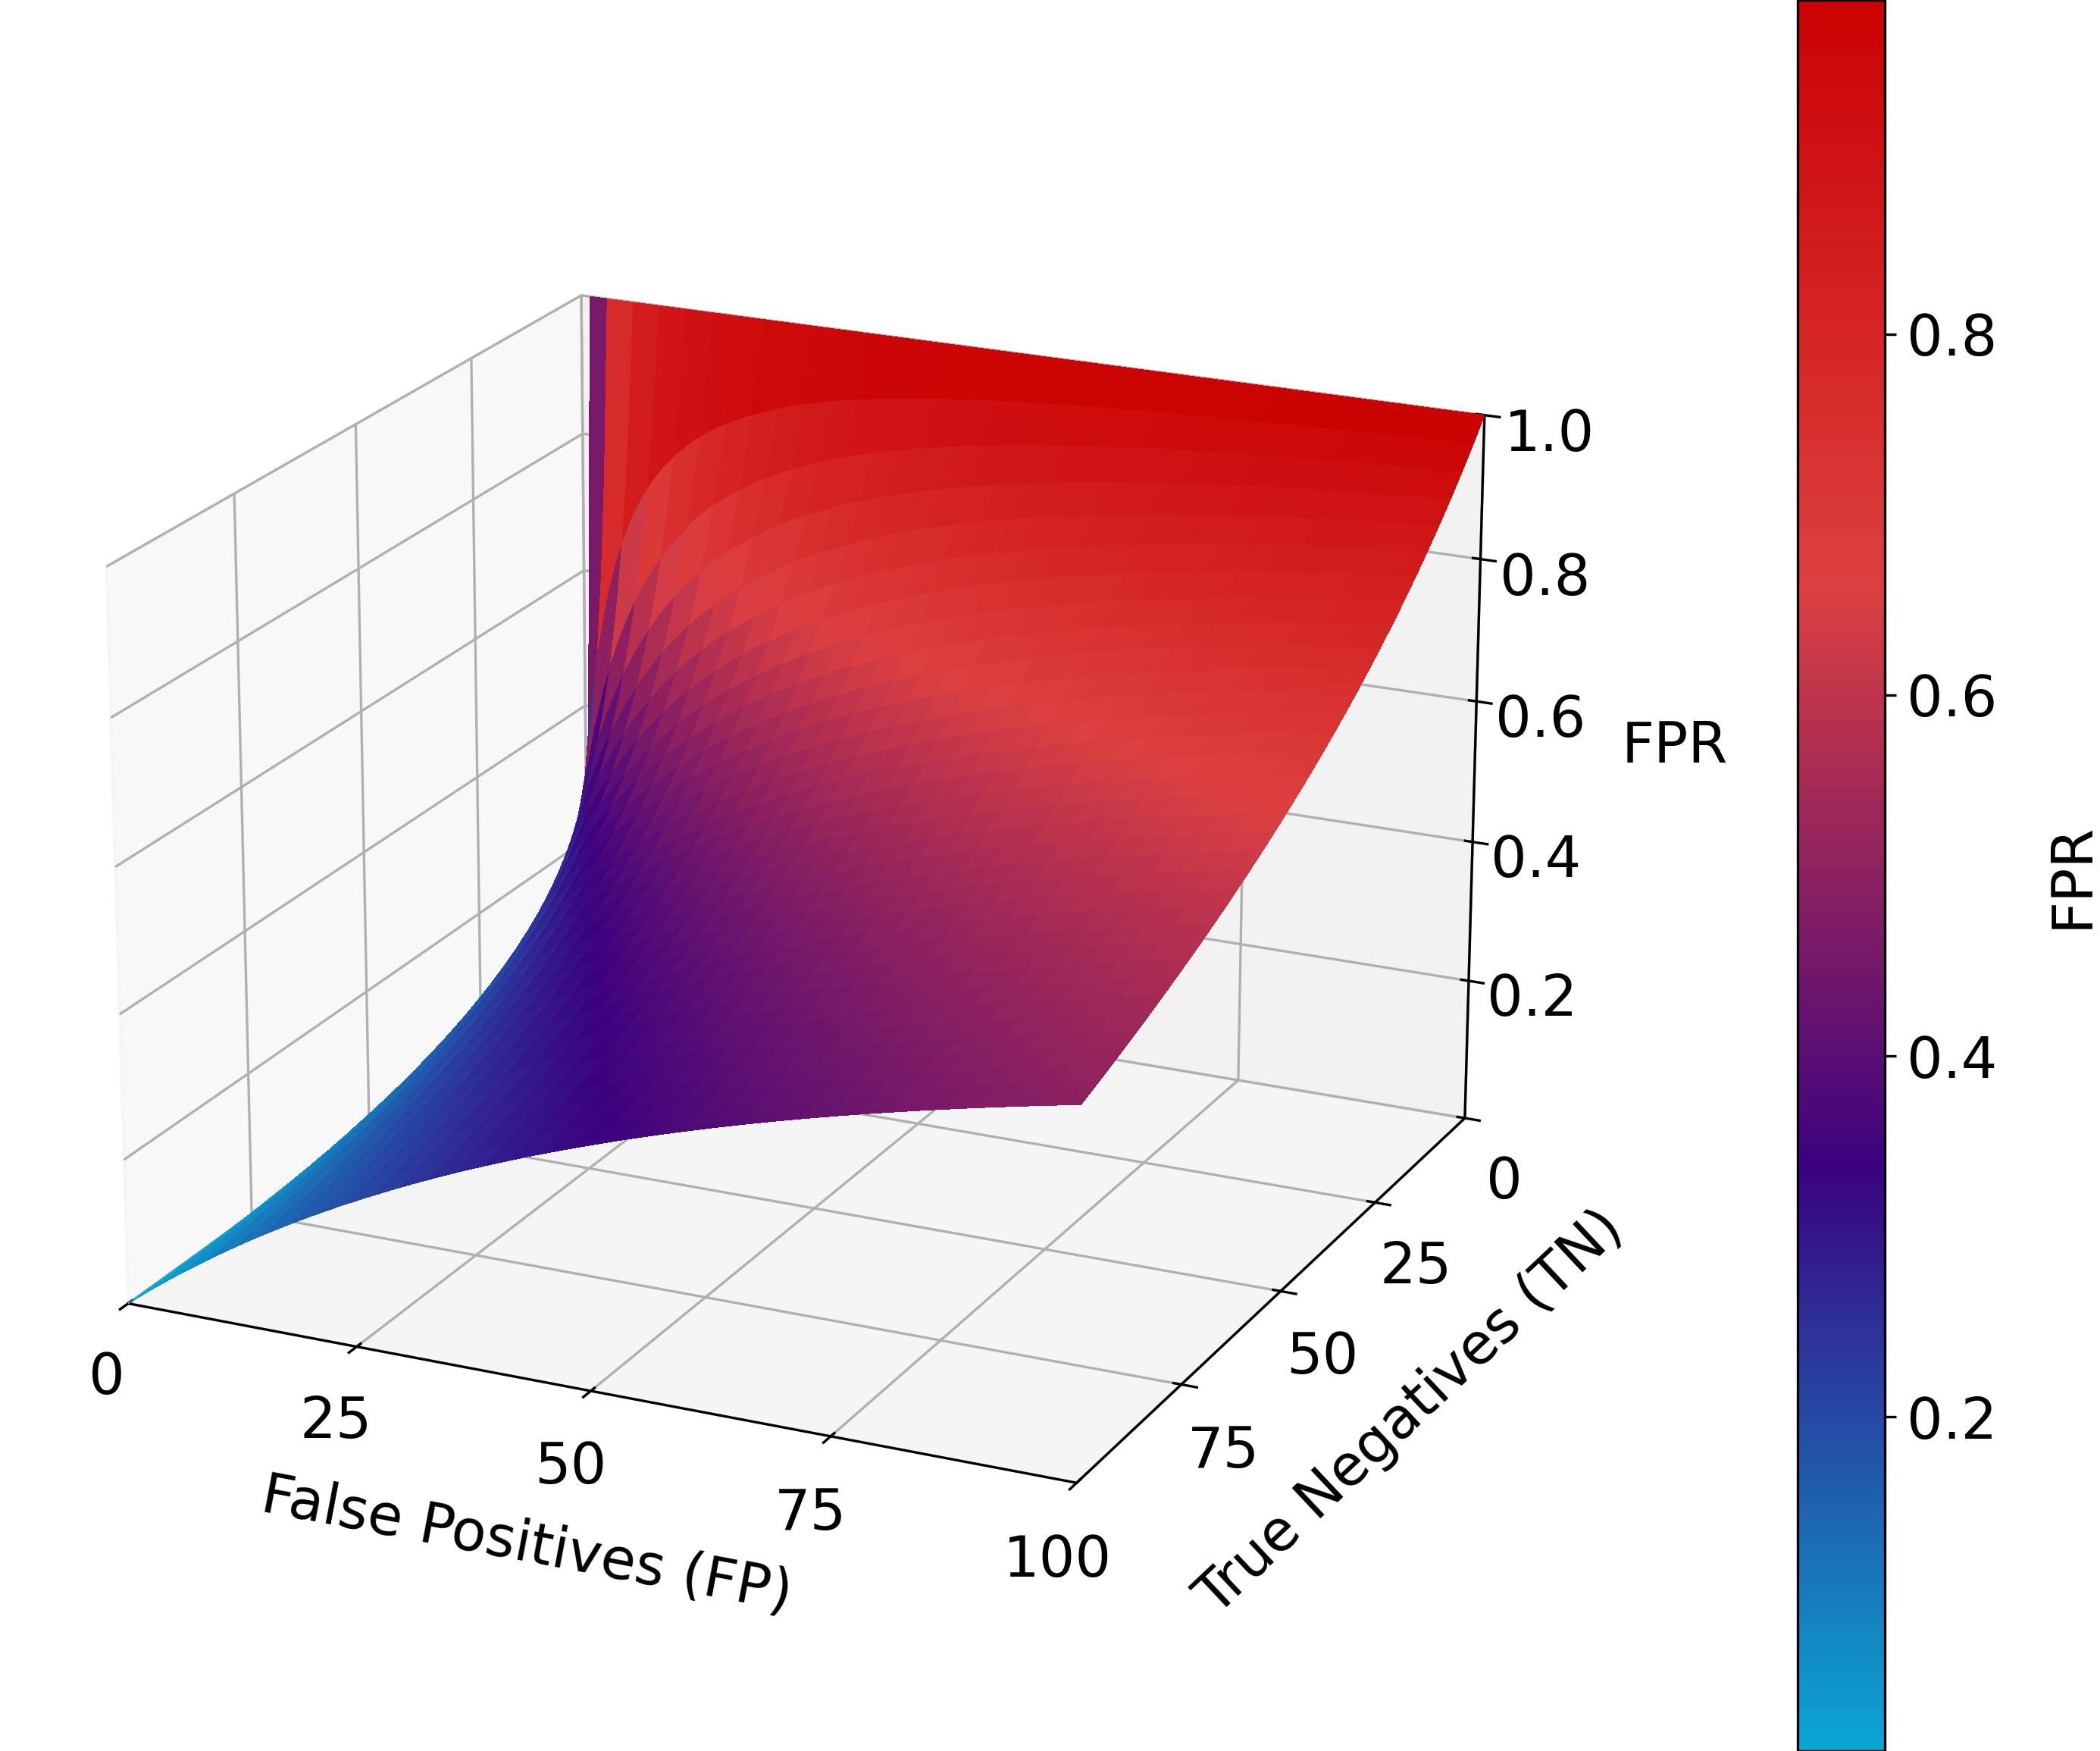
\includegraphics[width=0.7\textwidth]{figures/FPR_3d_surface.png}
    % \caption{Caption}
    \label{fig1}
\end{figure*}

\begin{wrapfigure}{r}{0.55\textwidth}
    \centering
    \vspace{-20pt} % Adjust vertical alignment if needed
    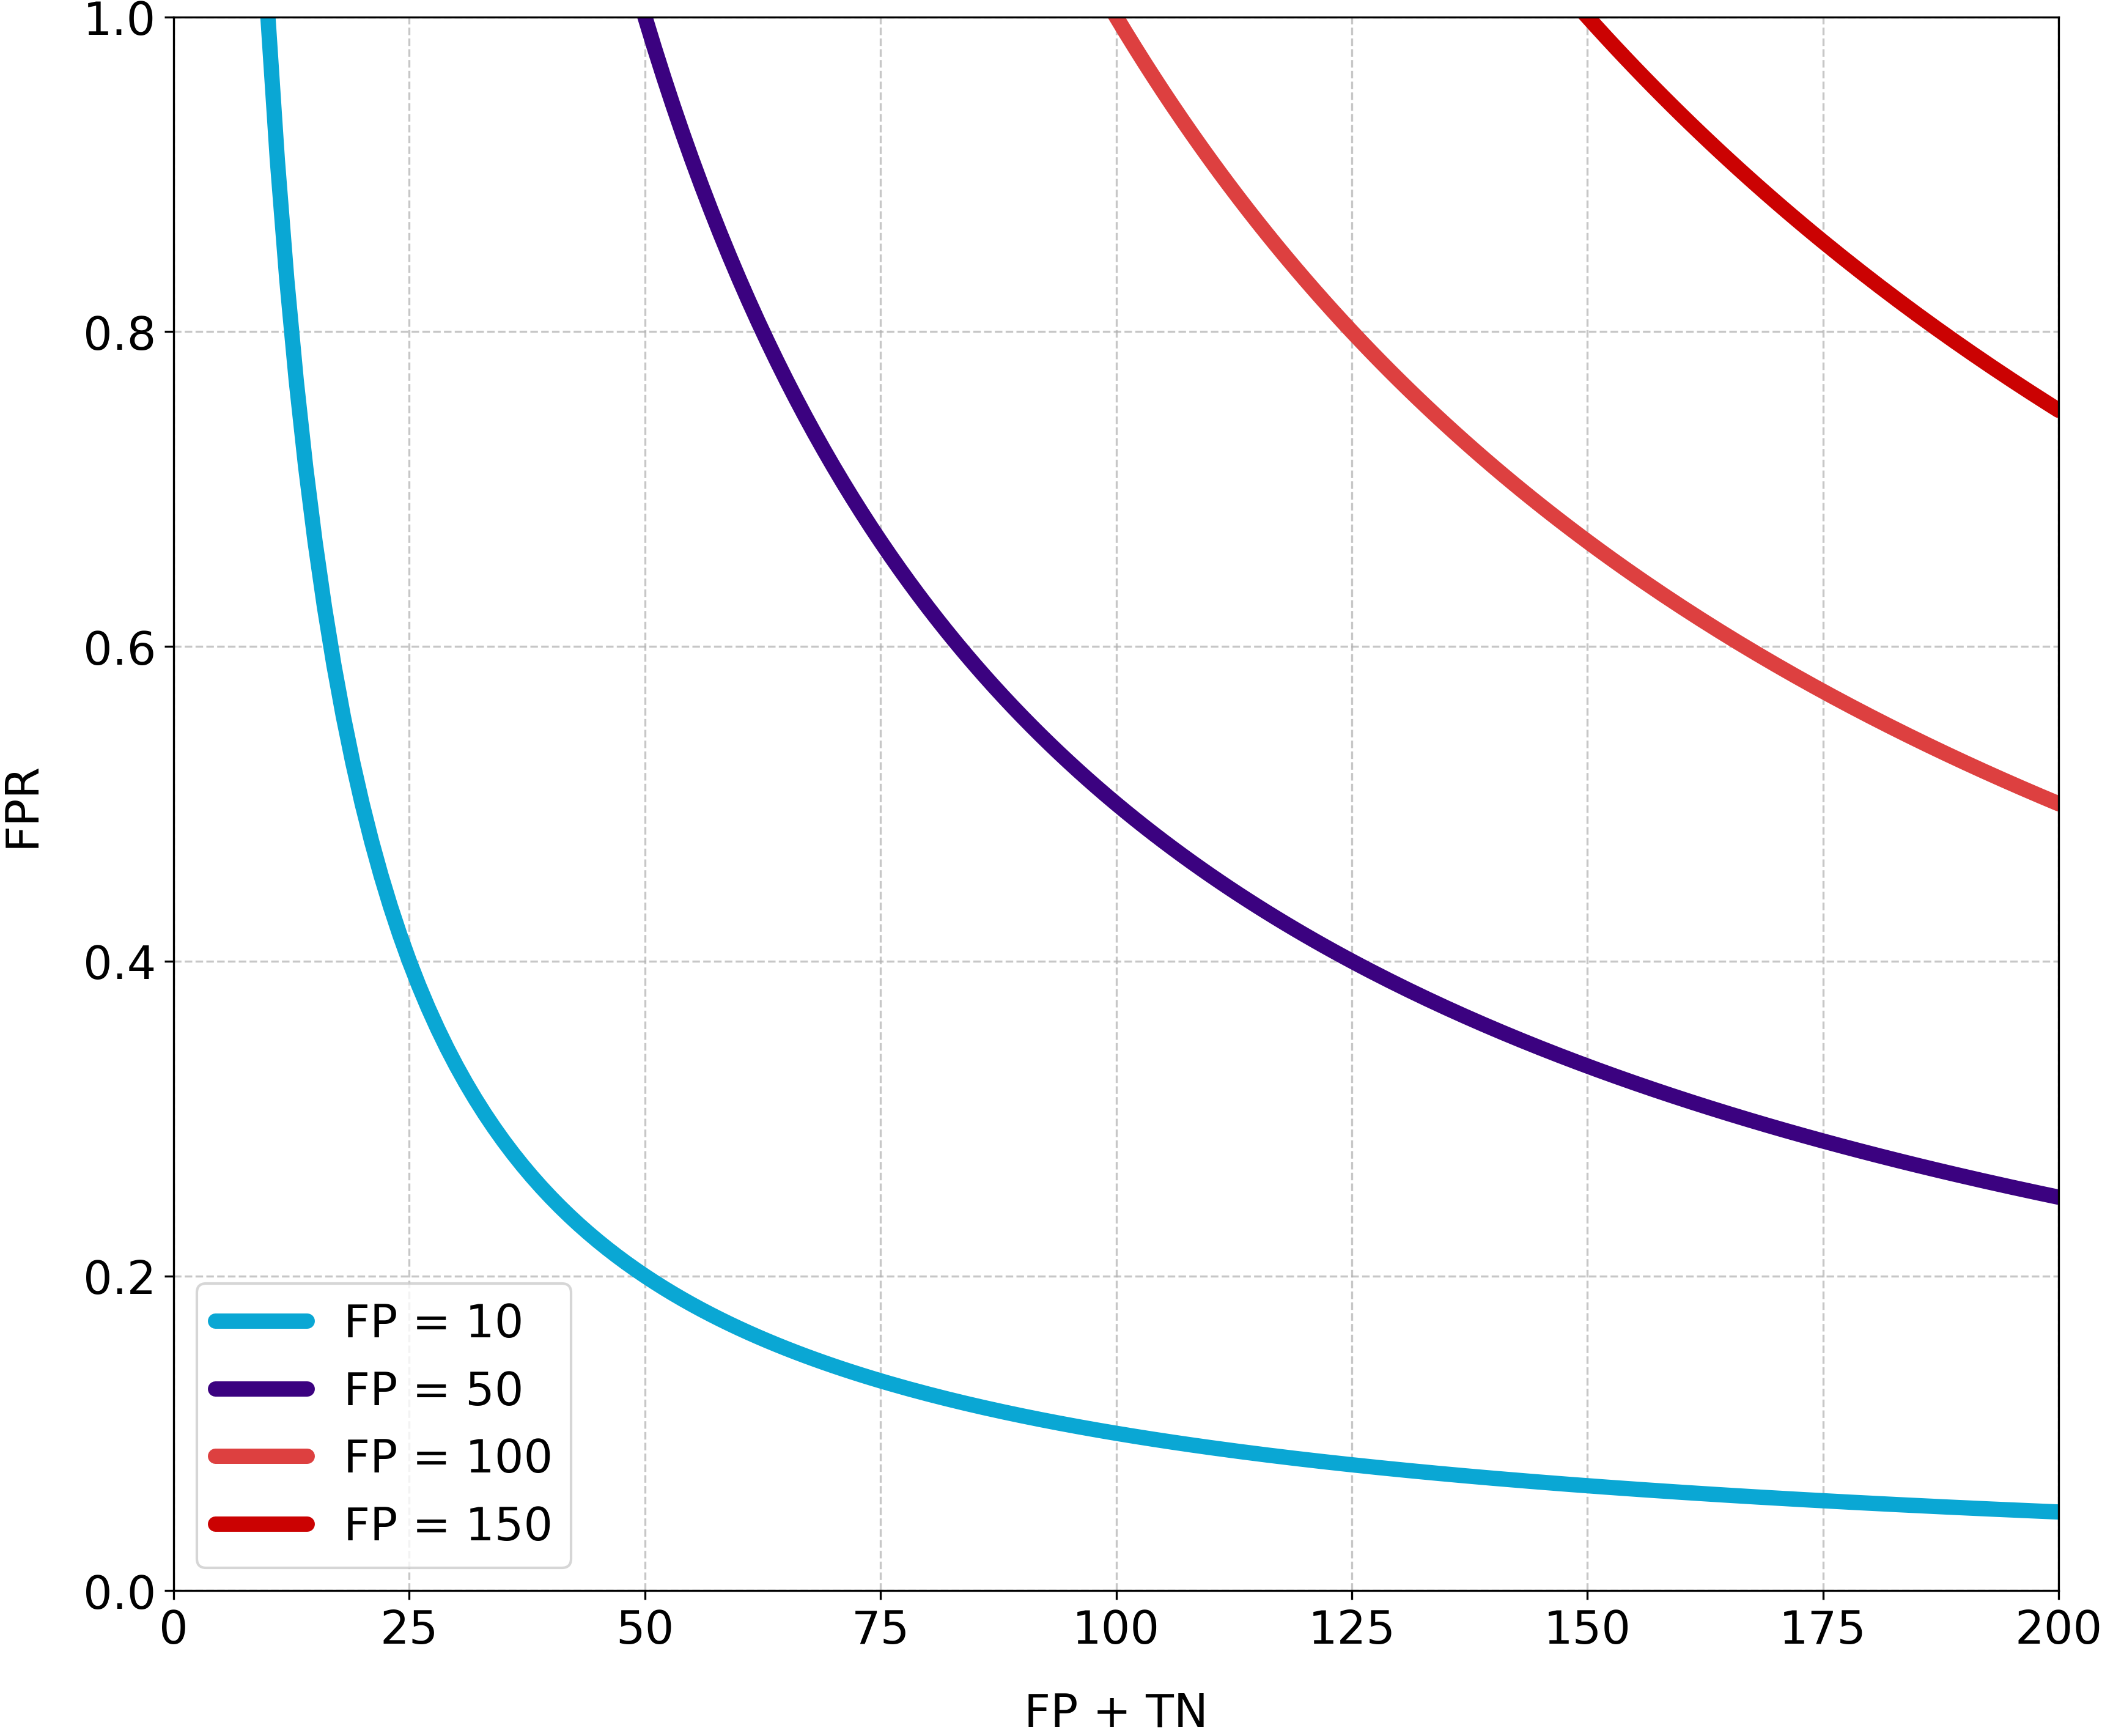
\includegraphics[width=0.5\textwidth]{figures/FPR_2d_line_plot.png} % Your figure goes here
\end{wrapfigure}

% Left text with the image on the right
\textbf{Figure 3.1 False Negative Rate.} 
\textbf{Top:}
3D surface illustrating FPR's non-linear relationship with FP and TN. FPR is lowest (blue) when FP is low. It increases (red) as FP increases.
\textbf{Right:}
Shows how FPR decreases hyperbolically as total negative cases increase for fixed FP values. Lower FP maintains better FPR.


\orangebox{%
Did you know that...}
{
    In hypothesis testing, reducing the False Negative Rate ($\beta$) increases the power of the test ($1 - \beta$), but often at the cost of increasing the False Positive Rate ($\alpha$).
    This demonstrates the inherent trade-off between Type I and Type II errors in statistical testing.
}

\textbf{FPR alternatives and related metrics}

Other metrics used alongside or instead True Positive Rate (TPR/Recall/Sensitivity), Specificity, Precision, F1-Score, and ROC curve.

% ---------- FNR ----------
\clearpage
\thispagestyle{classificationstyle}
\section{FNR}
\subsection{False Negative Rate}

% ---------- TPR ----------
\clearpage
\thispagestyle{classificationstyle}
\section{TPR}
\subsection{True Positive Rate (Recall/Sensitivity)}

% ---------- TNR ----------
\clearpage
\thispagestyle{classificationstyle}
\section{TNR}
\subsection{True Negative Rate (Specificity)}

% ---------- Accuracy ----------
\clearpage
\thispagestyle{classificationstyle}
\section{Accuracy}
\subsection{Accuracy}

% ---------- Balanced Accuracy ----------
\clearpage
\thispagestyle{classificationstyle}
\section{Balanced Accuracy}
\subsection{Balanced Accuracy}

% ---------- Precision ----------
\clearpage
\thispagestyle{classificationstyle}
\section{Precision}
\subsection{Precision}

% ---------- F1-score ----------
\clearpage
\thispagestyle{classificationstyle}
\section{F1-score}
\subsection{F1-score}

% ---------- F-beta ----------
\clearpage
\thispagestyle{classificationstyle}
\section{F-beta}
\subsection{F-beta}

% ---------- F-beta ----------
\clearpage
\thispagestyle{classificationstyle}
\section{F-beta}
\subsection{F-beta}

% ---------- ROC AUC ----------
\clearpage
\thispagestyle{classificationstyle}
\section{ROC AUC}
\subsection{Area Under the Receiver Operating Characteristic Curve}

% ---------- PR AUC ----------
\clearpage
\thispagestyle{classificationstyle}
\section{PR AUC}
\subsection{Area Under the Precision-Recall Curve}

% ---------- Brier Score Loss ----------
\clearpage
\thispagestyle{classificationstyle}
\section{Brier Score Loss}
\subsection{Brier Score Loss}

% ---------- Log Loss ----------
\clearpage
\thispagestyle{classificationstyle}
\section{Log Loss}
\subsection{Log Loss}

% ---------- Jaccard Score ----------
\clearpage
\thispagestyle{classificationstyle}
\section{Jaccard Score}
\subsection{Jaccard Score}

% ---------- D2 Log Loss Score ----------
\clearpage
\thispagestyle{classificationstyle}
\section{D2 Log Loss Score}
\subsection{D2 Log Loss Score}

% ---------- P4-metric ----------
\clearpage
\thispagestyle{classificationstyle}
\section{P4-metric}
\subsection{P4-metric}

% ---------- Cohen's Kappa ----------
\clearpage
\thispagestyle{classificationstyle}
\section{Cohen's Kappa}
\subsection{Cohen's Kappa}

% ---------- Phi Coefficient ----------
\clearpage
\thispagestyle{classificationstyle}
\section{Phi Coefficient}
\subsection{Phi Coefficient}

% ---------- MCC ----------
\clearpage
\thispagestyle{classificationstyle}
\section{MCC}
\subsection{Matthew's Correlation Coefficient}

\end{document}